\subsection{Kiểm chứng đổi món và thu chênh lệch}
\begin{table}[htbp]\centering\small
\begin{tabularx}{\linewidth}{|p{.13\linewidth}|X|}\hline
\textbf{Ca} & \textbf{Điều kiện cần chứng minh}\\\hline
EX-01 & Đổi bằng giá chuyển credit, hoàn/giữ snapshot đúng, không tạo Payment giả.\\\hline
EX-02 & Đổi cao hơn chỉ thu delta qua VNPay, điểm chỉ tăng theo tiền mới.\\\hline
EX-03 & Món thấp hơn giá trị đã trả bị yêu cầu chọn lại; thiếu kho mới rollback toàn bộ.\\\hline
EX-04 & Đơn PREPARING không được đổi; khách không gọi API quyết định của quầy.\\\hline
EX-05 & Duyệt đổi và bắt đầu pha đồng thời không cùng thành công theo trạng thái cũ.\\\hline
EX-06 & Giá đổi trước gửi làm fingerprint cũ bị từ chối; giá đổi sau gửi không thay báo giá đã lưu.\\\hline
EX-07 & REQUESTED chặn pha; rút yêu cầu đúng version cho phép tiếp tục đơn cũ, version cũ bị chặn.\\\hline
EX-08 & Hàng đợi lọc/phân trang và quyền BARISTA được kiểm ở backend.\\\hline
\end{tabularx}\caption{Các ca kiểm chứng đổi món trong bộ payment-exchange}
\end{table}

Các kịch bản có tại \path{test/payment-exchange.e2e-spec.ts}, thuộc bộ hồi quy đã nêu ở mục~\ref{sec:inventory-tests}; không suy ra một kết quả chạy mới chỉ từ việc bổ sung tài liệu. Kiểm thử giao diện của bản vá 08 sử dụng fixture để kiểm chọn món/giỏ đổi, gửi yêu cầu và thao tác quầy. Ảnh dưới minh họa UI với dữ liệu thử, không phải bằng chứng thu tiền thật.

\begin{figure}[htbp]\centering
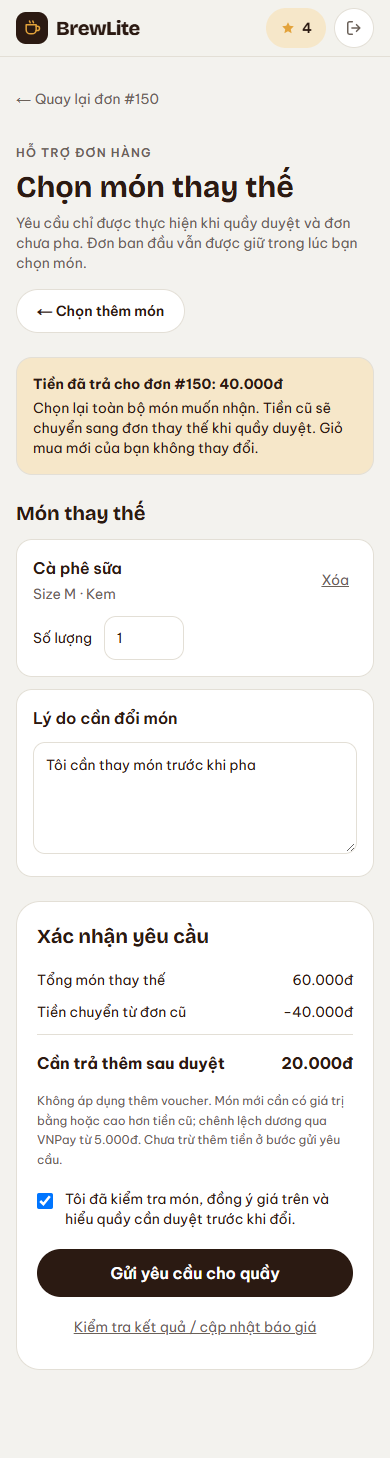
\includegraphics[width=.28\linewidth,height=.38\textheight,keepaspectratio]{assets/exchange/customer-cart-mobile.png}\hfill
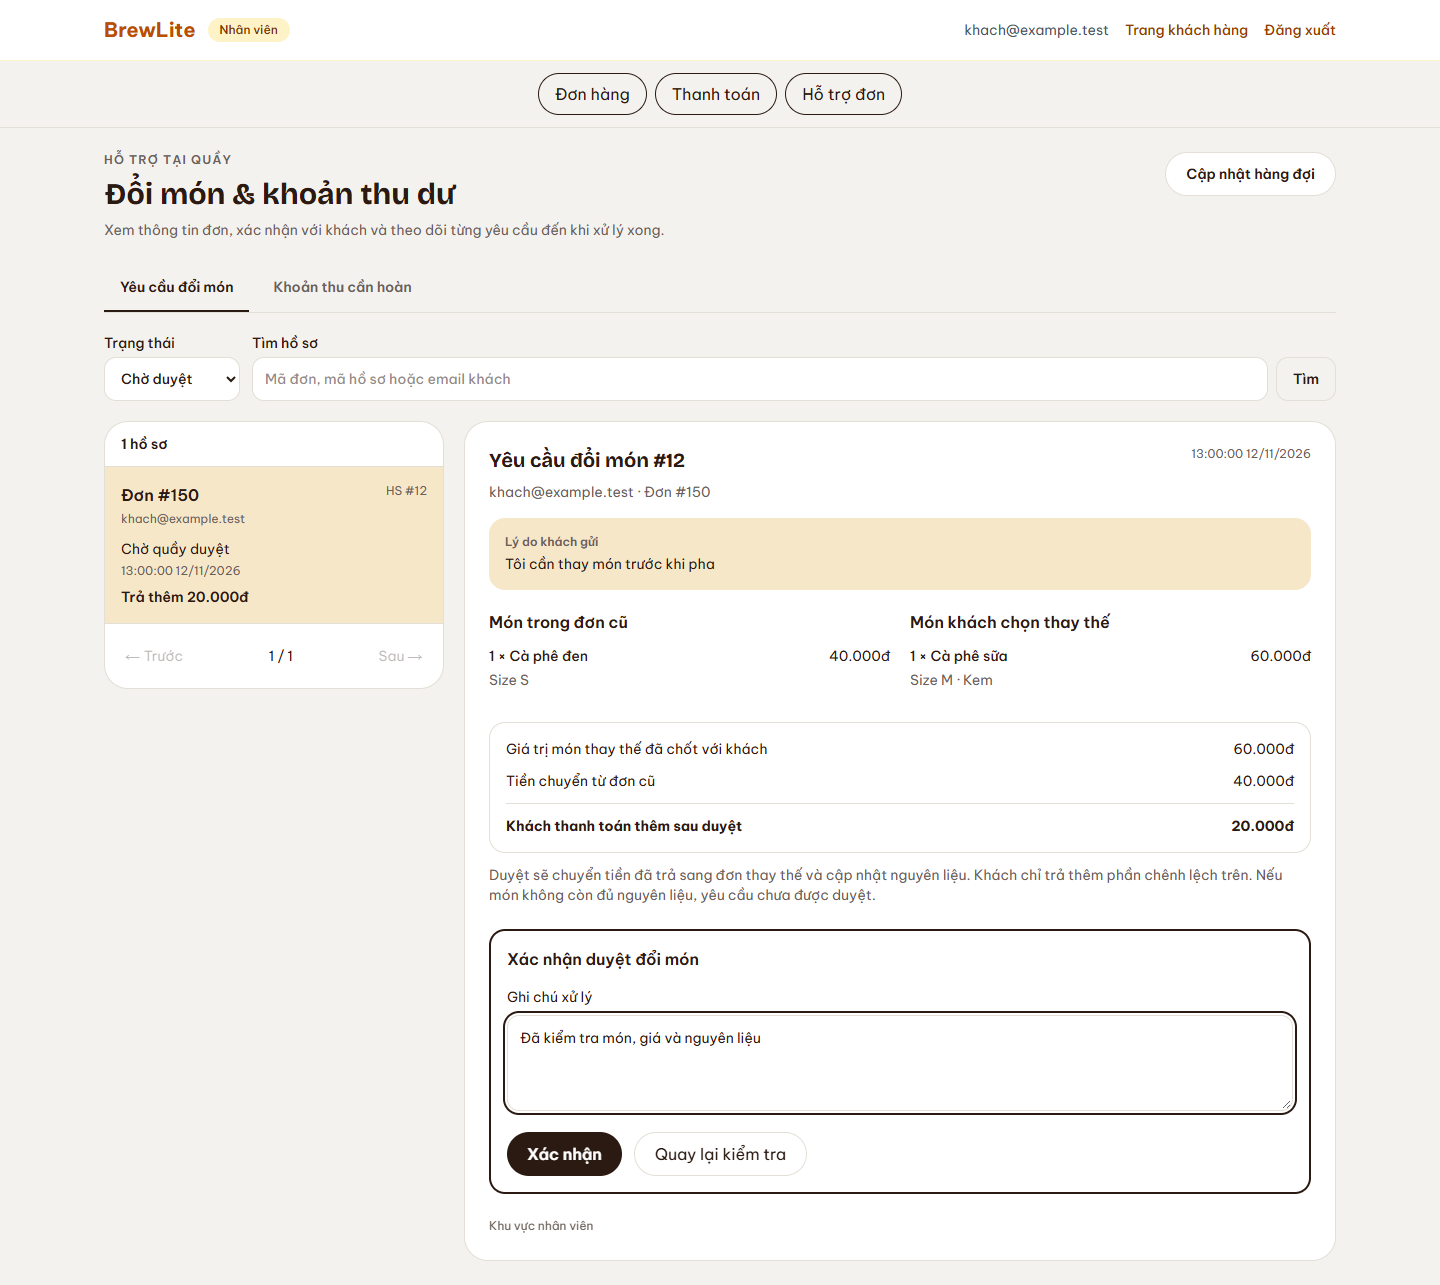
\includegraphics[width=.67\linewidth,height=.38\textheight,keepaspectratio]{assets/exchange/staff-exchange-desktop.png}
\caption{Giỏ đổi của khách và màn hình xử lý của barista (ảnh kiểm thử bằng fixture)}
\end{figure}
